W tej sekcji znajdziesz informacje na temat zarządzania różnymi ścieżkami dźwiękowymi w grze. Możesz kontrolować poziom głośności bezpośrednio z gry lub menu głównego, przechodząc do ustawień i przesuwając suwak od kontroli głośności muzyki lub osobnego suwaka dla reszty dźwięków. Ustawienia te są zapisywane w \texttt{PlayerPrefs}, co umożliwia utrzymanie preferencji gracza nawet po wyłączeniu gry. \\

\textbf{Kontrola głośności} jest również dostępna za pośrednictwem \textit{Audio Mixerów}. Modyfikacja zmiennych dostępnych w \texttt{PlayerPrefs} umożliwia kontrolę głośności z poziomu gry. Warto zauważyć, że te zmienne są udostępniane (zielone zaznaczenie po prawej na rysunku poniżej) do kontrolowania z \textit{Audio Mixerów} poszczególnych elementów dźwiękowych z poziomu skryptu, który obsługuje slidery głośności dostępne dla użytkownika w ustawieniach. \\

Oprócz tego, masz możliwość dostosowania głośności i efektów dźwiękowych z poziomu sceny. Modyfikowanie suwaków \textit{Audio Mixerów} od głośności (czerwone zaznaczenie na obrazku poniżej) lub suwaków komponentów \textit{Audio Source} na poszczególnych obiektach pozwala na precyzyjną kontrolę dźwięków w trakcie rozgrywki.

\begin{figure}[h]
    \centering
    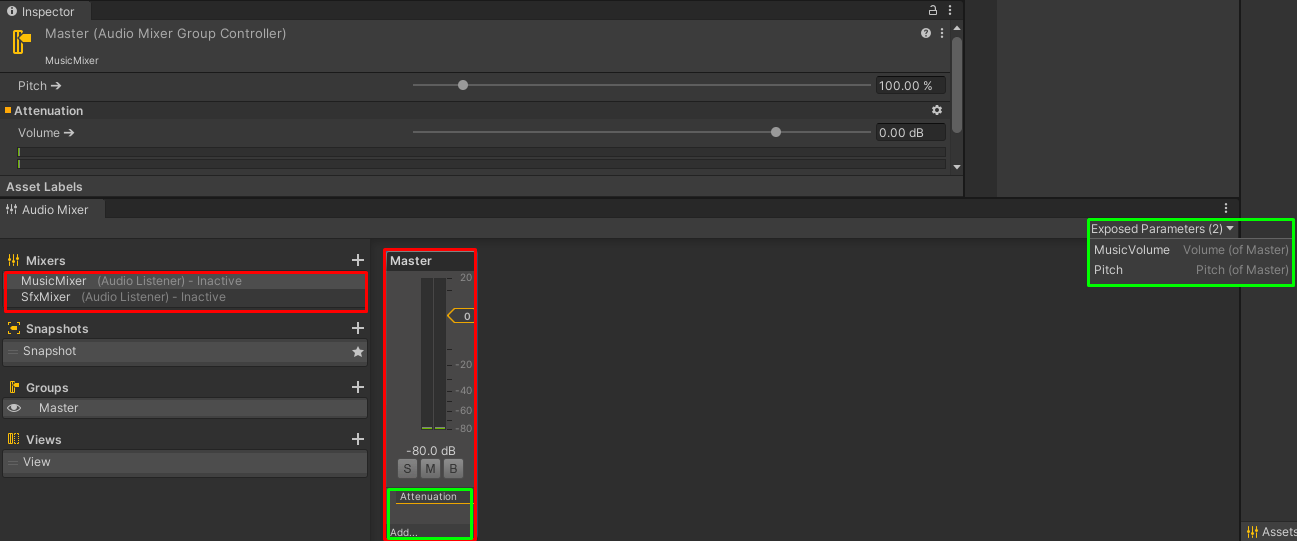
\includegraphics[width=1\linewidth]{Images/audioMixersSet.png}
    \caption{Ustawienia Audio Mixerów}
\end{figure}